\documentclass[]{article}
\usepackage{amsmath}
\usepackage{tabularx}
\usepackage{tikz}
\usetikzlibrary{positioning,automata,arrows}
\tikzset{
	->,  % makes the edges directed
	>=stealth, % makes the arrow heads bold
	node distance=1.2cm, % specifies the minimum distance between two nodes. Change if n
	every state/.style={thick, fill=gray!10}, % sets the properties for each ’state’ n
	initial text=$ $, % sets the text that appears on the start arrow
}

%opening
\title{}
\author{}

\begin{document}

\maketitle

\begin{abstract}

\end{abstract}

\section{Pictures}

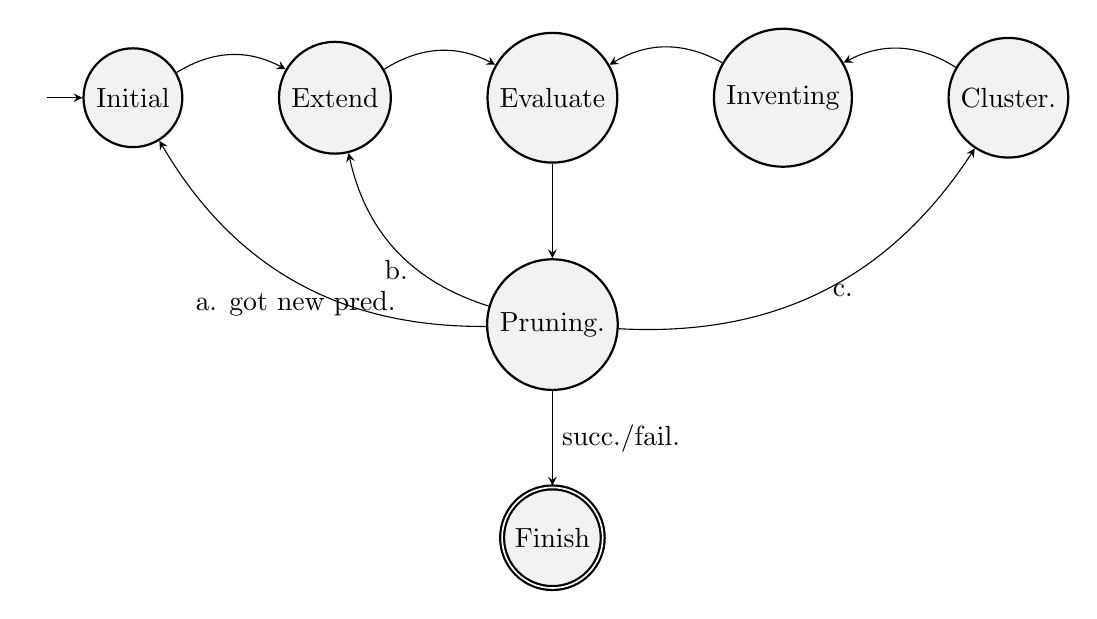
\begin{tikzpicture}[
	roundnode/.style={circle, draw=green!60, fill=green!5, very thick,rounded corners, minimum size=7mm},
	squarednode/.style={rectangle, draw=black!60, fill=black!0, very thick,rounded corners, minimum size=5mm},
	]
	%Nodes
		\node[state,initial]      (init)        {Initial};
	
	
	\node[state] (extension) [right=of init]	{Extend};
	\node[state] (eval) [right=of extension]	{Evaluate};	
	\node[state] (prune) [below=of eval]	{Pruning.};	
	\node[state, accepting]      (target)       [below=of prune]	 {Finish};

	\node[state]        (invent)       [right=of eval] {Inventing};	
	\node[state]        (cluster)       [right=of invent] {Cluster.};	

	%Lines
	\draw (init) edge[bend left, above] node{} (extension)
	 (extension) edge[bend left, above] node {} (eval)
	(eval) edge[right] node{} (prune)
	(cluster) edge[bend right,above] node{} (invent)
	(invent) edge[bend right, left] node{} (eval)
	(prune) edge[bend left, below] node{b.} (extension)
	(prune) edge[bend right,right] node{c.} (cluster)
	(prune) edge[right] node{succ./fail.} (target)
	(prune) edge[bend left, below] node{a. got new pred.} (init)
	 ;
	% \draw[->] (initclause.east) -- (language.west);
	% \draw[->] (language.south) -- (extended.north);
%	\path (extension) edge[loop above] node[anchor=north,above]{Self Extension} (extension);
\end{tikzpicture}


\end{document}
